\documentclass{beamer}
\usetheme{Pittsburgh}
\beamertemplatenavigationsymbolsempty


\usepackage{amsmath}
\usepackage{amssymb}
\usepackage{graphicx}

\usepackage{subfigure}
\usepackage{multirow}
\usepackage{multicol}
\usepackage{color}
\usepackage{url}
\usepackage{hyperref}
\usepackage{listings}
\usepackage{algorithm}
\usepackage{physics}
% add image path
\graphicspath{{../Images/}}

\title{Accelerating Numerical Simulations using Data-Driven Correction}
\author{Andrea Bonifacio}

\begin{document}

\begin{frame}
\titlepage
\end{frame}

\begin{frame}
\frametitle{Introduction}
\begin{itemize}
    \item The main drawback of numerical simulations is the computational cost.
    \item More accurate simulations \(\Rightarrow\) more computational cost.
    \item Idea: find a way to insert information from a more accurate simulation into a less accurate one.
\end{itemize}
\end{frame}

\begin{frame}
\frametitle{Goal}
\begin{columns}
    \column{0.5\textwidth}
    The ideal method should be:
    \begin{itemize}
    \item Geometry-independent.
    \item Topology-independent.
    \item Not a black-box.
    \item Fast.
    \end{itemize}
    \column{0.5\textwidth}
    The proposed method is:
    \begin{itemize}
    \item[] X
    \item[] \checkmark
    \item[] \checkmark
    \item[] \checkmark
    \end{itemize}
\end{columns}
\end{frame}

\begin{frame}
\frametitle{Methodology}
Consider a general boundary value problem:
\[
    \begin{split}
        \text{Find } u \text{ such that } \mathcal{L}u = f \text{ in } \Omega,\\
        B.C. \text{ on } \partial \Omega,
    \end{split}
\]
where \(\mathcal{L}\) is a differential operator, \(f\) is a source term, \(\Omega\) is the domain and \(\partial \Omega\) is the boundary of the domain. 

\vspace{0.5cm}
To solve it numerically, the domain is discretized into two meshes: a coarse mesh and a fine mesh. 
\end{frame}

\begin{frame}
\frametitle{Methodology}
\begin{itemize}
    \item The domain \( \Omega \) is discretized into two meshes \( \Omega_c \) and \( \Omega_f \) with \( n_c \) and \( n_f \) nodes respectively. 
    \item The solution associated with the fine mesh is denoted by \( u^f \) and the solution associated with the coarse mesh is denoted by \( u^c \).
    \item A set of points \(G \subset \Omega\) is chosen as a mutual grid for the two meshes.
    \item The solutions are interpolated on the mutual grid: \( u^f \approx u^f_G \) and \( u^c \approx u^c_G \).
    \item Now that both solutions live in the same space, the difference between them can be computed: \( e = u^f_G - u^c_G \).
\end{itemize}
\end{frame}

\begin{frame}
\frametitle{Methodology}
\begin{itemize}
    \item A dataset \(\mathcal{D} = \{u_G^c, e\}\) is created.
    \item A neural network is trained on the dataset.
    \item On a new simulation, the coarse solution is computed and its correction is obtained as: 
    \[
        \tilde{u}_G^c = u_G^c + \mathcal{NN}(u_G^c).
    \]
    \item Using RBF interpolation, the corrected solution is reconstructed on the mesh \( \Omega_c \):
    \[
        \tilde{u}^c = \text{RBF}(\tilde{u}_G^c).
    \]
\end{itemize}
\end{frame}

\begin{frame}
\frametitle{Pros and Cons}
\begin{columns}
    \column{0.5\textwidth}
    Pros:
    \begin{itemize}
        \item Avoid the black-box approach of other methods.
        \item Once trained on a single coarse mesh, the model works well even for different topologies.
        \item The small size of the model allows for fast computations.
    \end{itemize}
    \column{0.5\textwidth}
    Cons:
    \begin{itemize}
        \item This method is still geometry dependent.
        \item Needs a large dataset to train the model (for now).
    \end{itemize}
\end{columns}
\end{frame}

\begin{frame}
    \frametitle{Numerical Results}
    To test the method, two different linear elasticity problems were solved:
    \begin{itemize}
        \item A 2D beam
        \item A 3D beam
    \end{itemize}
    \begin{columns}
        \column{0.5\textwidth}
        \begin{figure}
            \centering
            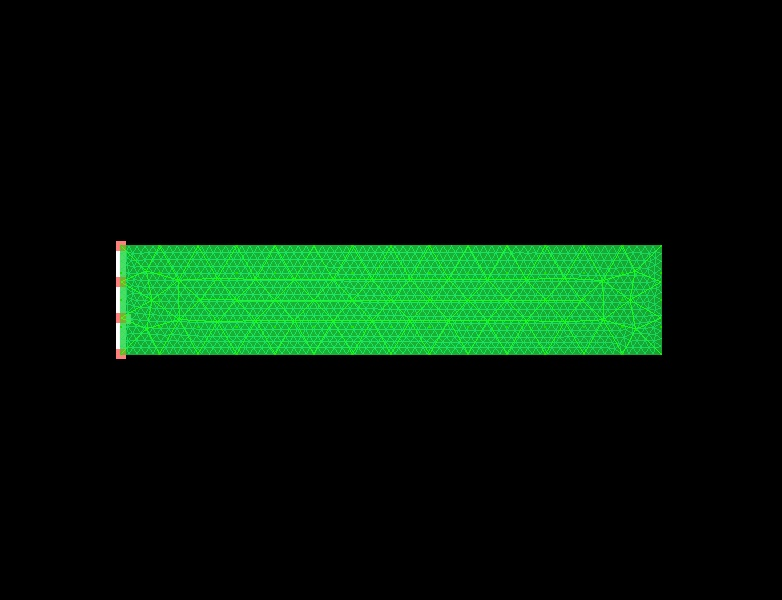
\includegraphics[width=0.8\textwidth]{Images/2D_beam.png}
            \caption{2D Beam}
        \end{figure}
        \column{0.5\textwidth}
        \begin{figure}
            \centering
            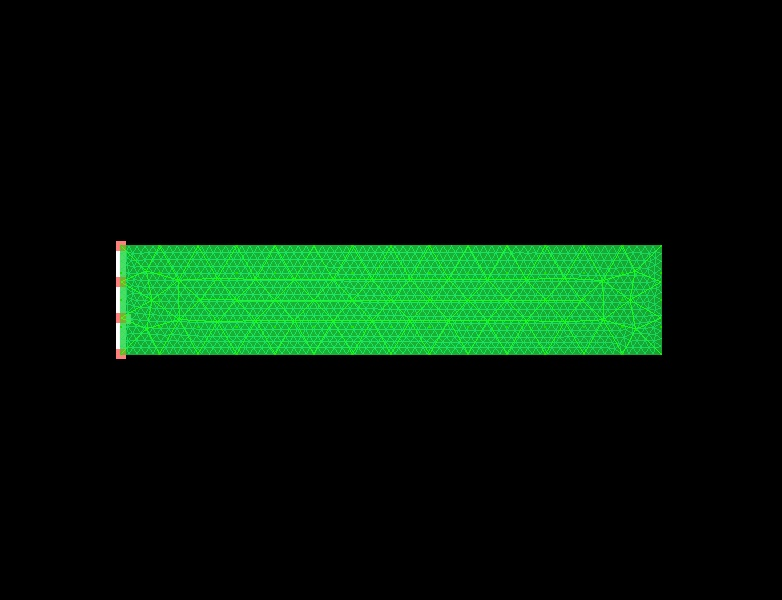
\includegraphics[width=0.8\textwidth]{Images/2D_beam.png}
            \caption{3D Beam}
        \end{figure}
    \end{columns}
\end{frame}

\begin{frame}
    \frametitle{Numerical Results - 2D Beam}
    In this case \( \Omega = [0, 10] \times [-1, 1] \) with Dirichlet boundary conditions on \(\{0\} \times [-1, 1]\) and a Neumann boundary condition on a random part of the remaining boundary.
    \vspace{0.5cm}

    The metric used to evaluate the performance of the method is the Root Mean Squared Error (RMSE) between the corrected solution and the fine solution.
    Here is a table with the results, testing the method on 100 different random simulations:
    \begin{table}
        \centering
        \begin{tabular}{|c|c|}
            \hline
            RMSE & 0.007981 ± 0.008958 m \\
            Extrema & 0.000255 \(\rightarrow\) 0.06638 m \\
            \hline
        \end{tabular}
    \end{table}
\end{frame}

\begin{frame}
    \frametitle{Numerical Results - 2D Beam}
    Here is an example of the corrected solution for a random simulation colored by the error:
    \begin{figure}
        \centering
        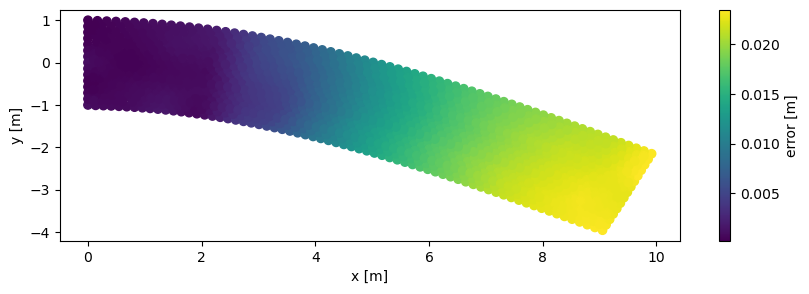
\includegraphics[width=0.8\textwidth]{Images/output_2D_beam.png}
    \end{figure}
\end{frame}

\begin{frame}
    \frametitle{Numerical Results - 3D Beam}
    In this case \( \Omega = [0, 10] \times [-1, 1] \times [-1, 1] \) with Dirichlet boundary conditions on \(\{0\} \times [-1, 1] \times [-1, 1]\) and a Neumann boundary condition on a random part of the remaining boundary.
    \vspace{0.5cm}

    The metric used to evaluate the performance of the method is the Root Mean Squared Error (RMSE) between the corrected solution and the fine solution.
    Here is a table with the results, testing the method on 100 different random simulations:
    \begin{table}
        \centering
        \begin{tabular}{|c|c|}
            \hline
            RMSE & 0.007981 ± 0.008958 m \\
            Extrema & 0.000255 \(\rightarrow\) 0.06638 m \\
            \hline
        \end{tabular}
    \end{table}
\end{frame}

\begin{frame}
    \frametitle{Numerical Results - 3D Beam}
    Here is an example of the corrected solution for a random simulation colored by the error:
    \begin{figure}
        \centering
        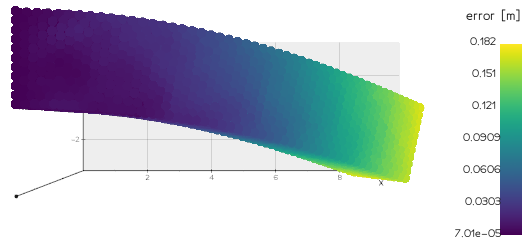
\includegraphics[width=0.8\textwidth]{Images/output_3D_beam.png}
    \end{figure}
\end{frame}

\begin{frame}
    \frametitle{Dynamic case}
    The final goal is to extend the method to the dynamic case. In that case some problems arise.
    \begin{itemize}
        \item Differences accumulate over time.
        \item The static model is not able to capture the dynamic behavior.
        \item How to capture data?
    \end{itemize}
    When the dynamic system behaves similarly to the static one, the static model works reasonably well.
\end{frame}

\begin{frame}
    \frametitle{Dynamic case - Ideas}
    Some ideas for the dynamic case:
    \begin{itemize}
        \item Create a new dataset containing both the solution and its time derivative, but keeping the same error as target.
        \item Creating two different datasets: one for the solution and one for the time derivative.
        \item Use a different network architecture capturing the time evolution. (But that would mean creating a black-box model).
    \end{itemize}
\end{frame}

\begin{frame}
    \frametitle{Conclusions}
    \begin{itemize}
        \item The method works well for static problems (given a suitable dataset).
        \item Maybe there is a way to efficiently sample the dataset.
        \item Probably GNNs could further improve the results (slower computations?).
        \item The dynamic case has still some open questions.
    \end{itemize}
\end{frame}
\end{document}

